% Vorlage Studien- und Diplomarbeiten, Bachelor- Masterarbeiten
%
% author: FG EMSP TU Berlin, Dipl.-Ing. Alexander Vorwerk
%
% last updated: 11.01.2011, by FG EMSP TU Berlin, Dipl.-Ing. Dennis lerch

% PREAMBLE, for use with pdfTex
% before documentclass
% disable pdfoutput to be able to include eps graphics and use packages like pstricks
% conversion dvi2ps and ps2pdf needed afterwards, pdftex specials like hyperref are still possible
%\pdfoutput=0														% dvi output - use with pdfcprot (character protruding)

\RequirePackage{fix-cm} 											% error correction for standard fonts

%% define CLASS
\documentclass[11pt, a4paper, parskip=half*, bibliography=totoc, cleardoublepage=empty, final,
numbers=noenddot]{scrbook} 											% begin every chapter one left page
% \documentclass[11pt, a4paper, parskip=half*, bibliography=totoc, cleardoublepage=empty, final,
% numbers=noenddot]{scrreprt}										% ongoing pages, no page break after chapter

%% misc
%\usepackage{cmbright}												% serifenlose computer modern fonts
\usepackage[T1]{fontenc}											% T1 fonts f�r gute pdf-Ausgabe
\usepackage[ansinew]{inputenc}										% wegen deutschen Umlauten
\usepackage[automark]{scrpage2}										% Koma Headers
\usepackage{fixltx2e}												% fixes for latex2e

% prepare for german AND english, last language loaded is default
%\usepackage[ngerman, english]{babel}								% switch by \begin{otherlanguage}{ngerman}.. \end{otherlanguage}
\usepackage[english, ngerman]{babel}								% switch by \begin{otherlanguage}{english}.. \end{otherlanguage}

\usepackage{boxit}	 												% frame handling
\usepackage{nag}													% warn user on outdated packages
\usepackage[linktocpage]{hyperref}									% links in pdf, thumbnails
\usepackage{soul}													% emphasizing text, underlining
\usepackage{breakurl}												% for broken urls in Bibliography when hyperref is in use
%\usepackage[square]{natbib}										% andere Literaturverweise, z. B. Zahlen
\usepackage[onehalfspacing]{setspace}								% 1.5, change line spaces by \singlespacing \doublespacing

%% tables
\usepackage{multicol} 												% multiple columns in tables
\usepackage{multirow}												% multiple rows in tables
\usepackage[margin=10pt,labelfont=bf]{caption}						% table headers
\usepackage{hhline}													% horizontal lines
\usepackage{longtable}												% pagebreak tables
\usepackage{booktabs}												% bold table lines, e.g. \toprule
\usepackage{tabularx}												% neue Tabular-Umgebung

%% math, symbols
\usepackage{amsmath}												% AMS Math like brackets, integrals...
\usepackage{amssymb}  												% AMS-Symbols v2.0
\usepackage{fixmath}												% big greek letters italic in math mode
\usepackage{array}													% matrices
\usepackage{units}		  											% includes nicefrac, nicer fracs for one line, SI-Units
\usepackage{trfsigns}												% symbole f�r transformationen
\usepackage{textcomp}												% einfache Sonderzeichen, z.B. \texteuro
\usepackage{gensymb}												% correct greek letters in units,\micro instead of \mu
\usepackage[integrals]{wasysym}										% for integrals like \oiint
\usepackage[version=3]{mhchem}										% easy typesetting of chemical formulae
\usepackage{ziffer}													% let"',"' be a valid delimiter in formulaes
\usepackage{dsfont}													% f�r andere Mengenzeichen, $\mathds{ABCDEFGHIJKLMNOPQRSTUVWXYZ}$

%% graphics
%\usepackage[activate]{pdfcprot}									% use margin kerning (character protruding) (Opt. Randausgleich)
\usepackage{microtype}												% character protruding, font expansion - instead of pdfcprot
\usepackage{graphicx}												% include graphics
\usepackage{wrapfig} 												% graphics in text
\usepackage{floatflt}												% graphics/tables in text
\usepackage{rotating} 												% rotating elements
\usepackage{listings}												% for programming source code
\usepackage[svgnames]{xcolor}										% colors for listings
\usepackage{psfrag}													% Text in .eps Grafiken ersetzen

%% layout
\usepackage[top=2.5cm,left=3.5cm,right=2.5cm,bottom=3cm]{geometry}

%%%%%%%%%%%%%%%%%%%%%%%%%%%%%%%%%%%%%%%%%%%%%%%%%%%%
% document definitions, do not change
% Allgemeine Schalter - �nderung von Standardeinstellungen
\frenchspacing																			% keine l�ngeren Leerzeichen nach Satzende/Abk�rzungen mit Punkt
\setlength{\parindent}{0pt}													% kein Einzug bei neuem Absatz
\setlength{\parskip}{1.5ex plus0.5ex minus 0.5ex}	  % Abstand zwischen 2 Abs�tzen

% verwende das paket setspace statt baselinestretch, Vorteil: Abst�nde in Fu�zeilen und
% listenumgebungen etc. bleiben erhalten
%\renewcommand{\baselinestretch}{1.2}								% Zeilenabstand

% Wortabst�nde optimal einstellen (use instead of \sloppy) - Verhindern von rausragenden Zeilen
\tolerance 1414
\hbadness 1414
\emergencystretch 1.5em
\hfuzz 0.3pt
\widowpenalty=10000
\vfuzz \hfuzz
\raggedbottom
\brokenpenalty=10000																% Trennung bei Seitenumbruch

\setlength{\headheight}{1cm} 												% H�he der Kopfzeile
\addtolength{\footnotesep}{2pt}											% abstand der Fu�note zur Trennlinie

% Setze �berschriftentiefe
\setcounter{secnumdepth}{3}													% Nummerierung der Kapitel
\setcounter{figure}{4}															% Bilder
\setcounter{tocdepth}{3}														% Gliederungsebene f�r Inhaltsverzeichnis

% Einstellungen f�r Kopf- und Fu�zeilen
\pagestyle{scrheadings}       % nutze scrheader
\clearscrheadings             % l�sche alle vorhandenen header

%\addtokomafont{pagehead}{\normalsize\upshape}  % nichtkursive Kopf-/Fu�zeilen
\setheadsepline{.05pt}					% trennlinie oben
\setfootsepline{.05pt}					% trennlinie unten


\automark[section]{chapter}   % links chapter, rechts section

% variere nach ein-/zweiseitig
\makeatletter
\if@twoside											% bei zweiseitig
	\lehead{\leftmark}            % setze Kapitel linke Seite oben
	\rohead{\rightmark}           % setze Abschnitt rechte Seite oben
	\lefoot{\pagemark}            % Seitennummer unten links
	\rofoot{\pagemark}            % Seitennummer unten rechts
	\lofoot{\Autor}       				% Name des Verfassers nur linke Seite
\else														% einseitig
	\ihead{\leftmark}            	% setze linke kopfzeile
	\ohead{\rightmark}           	% setze rechte kopfzeile
	\ofoot{\pagemark}             % seitennummer unten rechts
	\ifoot{\Autor}       					% Name des Verfassers unten links
\fi

% Bei Kapiteln ohne Subsection wird Kapitelname eingeblendet, nutze
% \markright{}, um den \rohead freizulassen

\makeatother




         								% input only replaces text, include creates newpage

%%%%%%%%%%%%%%%%%%%%%%%%%%%%%%%%%%%%%%%%%%%%%%%%%%%%
% user definitions, change this!
%%%%%%%%%%%%%%%%%%%%%%%%%%%%%%%%%%%%%%%%%%%%%%%%%%%%
% TO CHANGE
% path and extension of graphics, to be continued
\graphicspath{{./Titelblatt/}{./Kapitel1/Bilder/}{./Kapitel2/Bilder/}{./Kapitel3/Bilder/}}
\DeclareGraphicsExtensions{.eps}

% author, title, date of thesis 
\newcommand*{\Title}{Entwicklung eines 3D-Ultraschallger�tes}
\newcommand*{\Autor}{Hans Mustermann}
\newcommand*{\Datum}{Berlin, Mai 2007}
\title{\Title}
\author{\Autor} 
\date{\Datum}

% Beispiel f�r Definition neuer Kommandos f�r h�ufig gebrauchte Konstrukte
\newcommand{\tfk}[1]{\textsl{\texttt{#1}}}
\newcommand{\fett}[1]{\textbf{#1}}
\newcommand{\kursiv}[1]{\textit{#1}}
\newcommand{\pbb}{\parbox}
\newcommand{\sst}{\scriptstyle}

% f�r Standardumgebungen
%\renewcommand{\labelitemi}{*}												% Aufz�hlungszeichen definieren
   										% input only replaces text, includecreates newpage

%%%%%%%%%%%%%%% THESIS START %%%%%%%%%%%%%%
\begin{document}

	% Titelblatt
	%\thispagestyle{empty}
\begin{titlepage} 
\begin{centering}

	% Header
	\begin{figure}[!h]
		% TU Logo
  	\begin{minipage}{0.4\linewidth}
			\begin{center}
				
\includegraphics[scale=1]{tu-logo.eps} 
  		\end{center}  
  	\end{minipage}
		\hfill
		% EMSP Logo
  	\begin{minipage}{0.45\linewidth} 
  		\begin{center}
				
\includegraphics[scale=0.3]{Logo_final.eps} 
  		\end{center}    
  	\end{minipage}
	\end{figure}
	
	% vertikaler Zwischenraum
	\vspace{30mm}
	
	% Titel der Arbeit
	\LARGE

	Diplomarbeit
	
	\textbf{\Title}\\[2cm]

	
	\large
	erstellt von\\
	
	% Name des Verfassers
	\Autor\\
	Matrikel: 123456\\[3cm]

	% Betreuer
	\begin{minipage}{\linewidth} 
		\begin{tabbing}
    	Hochschullehrer:\quad \= Prof. Dr.-Ing. R. Orglmeister, TU Berlin\\
    	Betreuer:             \> Dr.-Ing. Sabine Musterfrau, Siemens AG \\
    						            \> Dipl.-Ing. Jens Exempel, TU Berlin \\
  	\end{tabbing}
  \end{minipage}
	
	% vertikaler Zwischenraum
	\vspace{20mm}
	
	\normalsize
	{Technische Universit�t Berlin, Fachgebiet Elektronik und medizinische Signalverarbeitung}\\
	{Institut f�r Energie- und Automatisierungstechnik}\\
	\Datum\\
\end{centering}
\end{titlepage}




	
										% F�ge Titelblatt ein
	\cleardoublepage												% Leere Seite
	\nocite{*}														% einbinden aller Literatureintr�ge

	% Vorspann
	\pagenumbering{roman}											% r�mische Seitennummerierung
	\tableofcontents 												% Inhaltsverzeichnis
	%Abk�rzungsverzeichnis
\chapter*{Abk�rzungen und Bezeichnungen}

\thispagestyle{empty}													% ohne Kopf und Fu�zeilen

% setzen des Tabs
\begin{tabbing}
-------------------\=--------------------------------\kill

% Abk�rzungen
AKF     \>Autokorrelationsfunktion\\
EKG     \>Elektrokardiogramm\\
FFT     \>Fast Fourier Transformation\\
VT      \>Versuchsteilnehmer\\

\end{tabbing}

\rule{10cm}{.3mm}
% Bezeichnungen

\begin{tabbing}
-------------------\=--------------------------------\kill

$P(A)$      \>Wahrscheinlichkeit f�r Ereignis A\\
$G$         \>Graph\\
$\mu$       \>Mittelwert\\

\end{tabbing}
								% Abk�rzungen
	% Erkl�rung
\thispagestyle{empty}													% ohne Kopf und Fu�zeilen
\begin{LARGE}
	\ul{\textbf{Erkl�rung}}
\end{LARGE}

\vspace{1cm}

Die selbst�ndige und eigenst�ndige Anfertigung versichert an Eides statt.
\vspace{2cm}

Berlin, den \today

\vspace{1cm}
%\rule{_Breite_}{_St�rke_}		%andersrum ist's vertikal

\rule{0.3\textwidth}{0.4pt}

Unterschrift

%\Datum
\vspace*{6cm}


									% Erkl�rung	(N�TIG!)
	% Danksagung

\begin{LARGE}
    \ul{\textbf{Danksagung}}		% package soul for underlining
\end{LARGE}

\vspace{1cm}

Der Autor dankt hiermit allen, die durch ihre Unterst�tzung zur
Entstehung dieser Arbeit beigetragen haben. Besonderer Dank gilt
vor allen Dingen den Betreuern seitens der Dingsbums AG, den
Damen und Herren Dr. Sowieso etc.

\newpage
									% Danksagung (optional) / acknowledgement
	\cleardoublepage

	% Hauptteil
	\pagenumbering{arabic}											% Umschalten der Numerierung / switch the numbering
	\chapter*{Kurzfassung}
\addcontentsline{toc}{chapter}{Kurzfassung}

Hier steht eine Zusammenfassung der Arbeit. Im Englischen wird f�r dieses Kapitel auch die
�berschrift ``abstract'' verwendet.

Der Unterschied zur ``Einleitung'' besteht darin, dass hier nicht der Aufbau der Arbeit, d.\,h.\ die
einzelnen Kapitel vorgestellt werden, sondern nur die bearbeitete Aufgabe und
Vorgehensweise kurz beschrieben und eine Zusammenfassung der Ergebnisse gegeben wird. Daher sollte
die ``Kurzfassung'' nicht l�nger als eine halbe Seite sein.
										% Kurzfassung der Arbeit / abstract of the thesis
	% Kapitel 1 - Einleitung

\chapter[Einleitung]{Einleitung} \label{chap:Einl}
\section[Teil Zwei]{Erster Teil} \label{sec:EinlTeil1}

Normale Aufz�hlung:
\begin{itemize}

	\item{Erstens}
	\item{Zweitens}
	\item{Drittens}

\end{itemize}

\subparagraph{Beispieltext}
Der Austausch von Information zwischen Systemen erfolgt mittels Signalen.
Das Signal kann als mathematische Funktion von einer oder mehreren unabh�ngigen
Variablen (z.\,B.\ Zeit, Raumkoordinaten) verstanden werden. Als Tr�ger des
Signals sind verschiedene physikalische oder auch chemische Gr��en denkbar, wie
z.\,B.\ Spannung, Strom, Druck, Lichtst�rke, Stoffkonzentration oder Temperatur.

Die Aufgabe der Signalverarbeitung besteht in der Manipulation, Analyse,
Interpretation und Darstellung von Signalen. Mit anderen Worten geht es darum,
den Verlauf der Signalfunktion gezielt zu ver�ndern. Dies kann beispielsweise
�ber die Ausblendung unerw�nschter, oder die Verst�rkung geforderter
Frequenzanteile im Signal erfolgen. H�ufig geht es auch um die Trennung
verschiedener im Signal enthaltener Anteile zur separaten Weiterverarbeitung. Die
praktische Realisierung lehnt sich, insbesondere im analogen Bereich der
Signalverarbeitung, stark an die physikalische Natur des Signaltr�gers (z.\,B.\
elektrische Filter, UV-Filter) an.

Die Signalverarbeitung hat sich in den letzten Jahrzehnten in vielen Bereichen
durchgesetzt und ist aus der modernen Technik nicht mehr wegzudenken. Gro�e
Einsatzgebiete liegen in der Medizintechnik, Nachrichtentechnik, Automatisierung,
Verfahrenstechnik, Bild- und Sprachverarbeitung, der Unterhaltungselektronik,
Funk und Navigation oder auch in der Autoindustrie. Im Prinzip findet
Signalverarbeitung heute in nahezu allen industriellen Bereich ihre Anwendungen.

Entwicklungsgeschichtlich bedingt haben sich zwei in ihrer Bedeutung
gleichberechtigte Zweige der Signalverarbeitung herausgebildet,

Aufz�hlung mit anderen Zeichen
\begin{itemize}
        \item[-] die analoge Signalverarbeitung und
        \item[-] die digitale Signalverarbeitung.
\end{itemize}

\section[Teil Zwei]{Zweiter Teil}\label{sec:EinlTeil2}
\subparagraph{Nochmal Text}
Die Signalverarbeitung hat sich in den letzten Jahrzehnten in vielen Bereichen
durchgesetzt und ist aus der modernen Technik nicht mehr wegzudenken. Gro�e
Einsatzgebiete liegen in der Medizintechnik, Nachrichtentechnik, Automatisierung,
Verfahrenstechnik, Bild- und Sprachverarbeitung, der Unterhaltungselektronik,
Funk und Navigation oder auch in der Autoindustrie. Im Prinzip findet
Signalverarbeitung heute in nahezu allen industriellen Bereich ihre Anwendungen.



	% Kapitel 2 - Mathe

\chapter{Mathematische Ausdr�cke und Formeln} \label{chap:math}
%%%%%%%%%%%%%%%%%%%%%%%%%%%%%%%%%%%%%%%%%%%%%%%%%%%%%%%%%%%%%%%%%%%%%%%%%%%%%%%%%%%%%%%%%%%%%%

%%%%%%%%%%%%%%%%%%%%%%%%%%%%%%%%%%%%%%%%%%%%%%%%%%%%%%%%%%%%%%%%%%%%%%%%%%%%%%%%%%%%%%%%%%%%%%
\section{Matrizen} \label{sec:matrizen}

Matrizen gehen so: TEST

Definition einer $(M \times N)$-Matrix:
\begin{equation}
	{\bf A}=\left(
		\begin{array}{cccc}
			a_{11}  & a_{12}        & \cdots                & a_{1N}        \\
			a_{21}  & a_{22}        & \cdots                & a_{2N}        \\
			\vdots  & \vdots        & \ddots                & \vdots        \\
			a_{M1}  & a_{M2}        & \cdots                & a_{MN}
		\end{array}
		\right)
		  =(a_{ij})
\end{equation}


\section{Schreibweisen und Formelsatz}

Oft stellt sich die Frage, ob man ein Formelzeichen oder einen Bezeichner in
einer Zeichnung senkrecht (also ``normal'' bzw. nicht-kursiv) oder
\textit{kursiv} zu schreiben hat. Um diese Fragen zu kl�ren folgen nun die
wichtigsten Regeln, wie sie Standard sein sollten. Sie sind aus den DIN-Normen
1338 und 1302 �bernommen. Zus�tzlich wird darauf hingewiesen, wie man in
mathematischen Formeln die korrekten Abst�nde zwischen den Elementen und
Einheiten einzuhalten hat.

Um zwischen mathematischen und physikalischen Konstanten und Variablen
unterscheiden zu k�nnen, werden diese mit unterschiedlichen Schreibweisen
gekennzeichnet.

\subsection{Senkrechte Schreibweise}
\textbf{Mathematische Konstanten} werden generell senkrecht geschrieben.
Dazu geh�ren beispielsweise die Euler�sche Zahl $\mathrm{e}$, die Zahl $\pi$ oder $	\mathrm{j}$ bzw. $	\mathrm{i} = \sqrt{-1}$. \textbf{Mathematische Funktionen und Operatoren} schreibt man senkrecht.
z.\,B.\ $\sin, \cos, \exp, \ln$ und  $\mathrm{\frac{d}{dt}}$

\subsection{Kursive Schreibweise}
\textbf{\textit{Physikalische Konstanten}}, die physikalische Gr��en bezeichnen werden generell \textit{kursiv} geschrieben.
z.\,B.\ $R, L$ oder $i, u$ und Konstanten wie $\epsilon_0$ oder $k$.

\textbf{\textit{Variablen}} werden generell kursiv geschrieben

\subsection{Schreibweise des Index}
F�r Indizes gelten dieselben wie oben beschriebenen Regeln:
Beschreiben die Indizes eine Variable, so werden sie kursiv geschrieben So schreibt man beispielsweise den Ohm�schen Widerstand $R$ einer Induktivit�t $L$: $R_L$. $R$ und $L$ bezeichnen beide physikalische Gr��en, und werden somit kursiv geschrieben.
Dient der Index jedoch der Bezeichnung der Funktion von bestimmten Elementen, so wird dieser senkrecht gedruckt. M�chte man beispielsweise einen Widerstand R als Lastwiderstand kennzeichnen, so geschieht dies mit einer senkrechten Indizierung: $R_{\mathrm{Last}}$
Z�hlvariablen, als oft vorkommendes Beispiel, werden als Ver�nderliche im Index ebenfalls kursiv geschrieben. Z.\,B.\ $k_n$ , wobei $n$ beispielsweise die Zahlen von $0 \ldots 10$ durchl�uft.
Ein bestimmtes Element z.\,B.\ von einem Vektor, wird jedoch mit senkrechten Zahlen indiziert. So z.\,B.\ $k_1$.

Der folgende Hinweis ist eigentlich unn�tig:
{\footnotesize Hinweis f�r Microsoft Word:
Neben der �blichen Formatierung �ber Men�befehle gibt es noch die M�glichkeit Shortcuts einzusetzen:
Soll ein Index hochgestellt werden, so bet�tigt man unter Festhalten der Ctrl- bzw. Strg- Taste die * - Taste. Jetzt kann man den gew�nschten Index eintippen.
Soll ein Index tiefgestellt werden, so dr�ckt man Ctrl bzw. Strg und \#.}

\section{Formelsatz}
\subsection[Formelabst�nde]{Korrekte Abst�nde in Formeln}
Man nutze z.\,B.\ den Befehl ``$\backslash$unit [2]\{kHz\}'': Das Ergebnis sieht dann immer so aus $f_1=\unit[2]{kHz}$. Der folgende Abschnitt er�brigt sich bei Benutzung von LaTeX. {\footnotesize MS Word: Um Formeln �bersichtlicher zu gestalten, soll zwischen allen Elementen ein festes Leerzeichen, also ein an den vorhergehenden Ausdruck gebundenes Freizeichen gelassen werden. In Microsoft Word und im Formeleditor erh�lt man ein solches Leerzeichen indem man die Space-Taste unter Gedr�ckthalten der Shift und der Ctrl- bzw. Strg-Taste bet�tigt.
Auf dem Bildschirm werden diese als Steuerzeichen ``$ \circ $'' sichtbar.
$R = \unit[100]{\Omega}$  ist als $R \circ = \circ \unit[100\circ]{\Omega}$ zu sehen. Diese Regelung ist besonders bei einheitengebundenen Zahlen wie in diesem Beispiel zu beachten. So muss zwischen Zahl und Einheit immer ein festes Leerzeichen gesetzt werden! Abgesehen von der �bersicht haben diese festen Leerzeichen den Vorteil, dass die Zahlen beim Zeilenumbruch nicht von ihrer Einheit getrennt werden.}

\normalsize
\newpage
\subsection[Formelbeispiel]{Beispiel f�r eine richtig dargestellte Formel}
Als Bild (aus Word):
\begin{figure}[!htbp]
			\begin{center}
				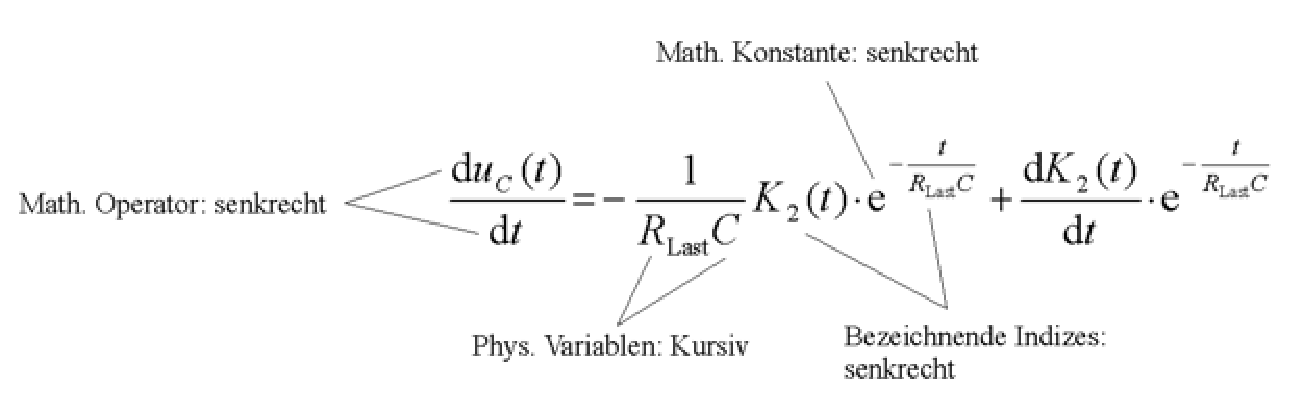
\includegraphics[scale=0.6]{formelbeispiel}
				\caption{Formelbeispiel}
				\label{kap2:formelbeispiel}
  		\end{center}
\end{figure}

Und nun in LaTeX als Formel:
\begin{equation}
		\frac{\mathrm{d}u_C(t)}{\mathrm{d}t}
		=	- \frac{1}{R_{\mathrm{Last}}C} K_2(t) \cdot \mathrm{e}^{-\frac{t}{R_{\mathrm{Last}}C}} 																	+ \frac{\mathrm{d}K_2(t)}{\mathrm{d}t} \cdot \mathrm{e}^{-\frac{t}{R_{\mathrm{Last}}C}}
		\label{kap2:eqformelbeispiel}
\end{equation}


\subsection{Weitere Formeln} \label{sec:formeln}
\subsubsection{Fouriertransformation}
\paragraph{Analyse}
Die Berechnung der Fouriertransformierten\footnote{So k�nnte eine Fu�note aussehen.} erfolgt mit der Analysegleichung:
\begin{equation}
	F(\mathrm{j}\omega)  = {\cal F}[f(t)] = \int\limits_{-\infty}^{\infty}f(t)\cdot \mathrm{e}^{-\mathrm{j}\omega t}\mathrm{d}t
	\label{analft}
\end{equation}

\paragraph{Synthese}
Die Synthesegleichung der Fouriertransformation lautet:

\begin{equation}
	f(t)  = \frac{1}{2 \pi}\int\limits_{-\infty}^{\infty}F(j \omega) \cdot \mathrm{e}^{\mathrm{j}\omega t}\mathrm{d}\omega
	\label{synthft}
\end{equation}

\subsubsection{weitere Transformationen}
Der mathematische Zusammenhang zwischen einer Zeitfunktion $f(t)$ und ihrer %%@
Laplacetransformierten $F(s)$ ist durch die Analysegleichung definiert:
\begin{equation}
	F(s) = {\cal L}[f(t)] := \int\limits_{-\infty}^{\infty}f(t)\cdot \mathrm{e}^{-st}\mathrm{d}t
	\label{anallaplace}
\end{equation}
Die komplexe Frequenz $s = \sigma +\mathrm{j}\omega$ wird in einem rechtwinkligen Koordinatensystem, der %%@
Laplace- bzw. $s$-Ebene, dargestellt.
%
%
\subsubsection{Gro�e griechische Buchstaben}
Sollen in einer Formel gro�e griechische Buchstaben verwendet werden, ist es n�tig, das Paket \textsl{fixmath} einzusetzen, da diese ansonsten nicht kursiv dargestellt werden, wenn es sich um Variablen handelt, z.\,B.:

Die normierte Kreisfrequenz ist gegeben als
%
\[\upOmega = 2\pi\frac{f}{f_t} = 2\pi\frac{\omega}{\omega_t} \qquad \text{ohne fixmath}\]
\[\Omega = 2\pi\frac{f}{f_t} = 2\pi\frac{\omega}{\omega_t} \qquad \text{mit fixmath}\]

\subsubsection{Weitere Pakete}
\paragraph{Griechische Buchstaben in Einheiten}
F�r die Verwendung von griechischen Buchstaben in Einheiten ist bei einigen Schriftarten das Paket \textsl{gensymb} notwendig:
%
\[\unit[5]{\mu V} \qquad \text{ohne gensymb}\]
\[\unit[5]{\micro V} \qquad \text{mit gensymb}\]

\paragraph{Erweiterte Integrale}
Das Paket \textsl{wasysym} liefert erweiterte M�glichkeiten f�r den Satz von Integralen, z.\,B.\ f�r Oberfl�chenintegrale mit mehreren Integralzeichen:
%
\[\oiint\limits_{A_Q}{\vec{G}(\vec{r}) dA_Q}\]

\paragraph{Chemische Formeln}
Mit Hilfe des Paketes \textsl{mhchem} lassen sich einfach chemischen Formelzeichen bzw.\ Formeln setzen:
%
\[\ce{Na+} \quad \ce{O^2-} \quad \ce{H2CO3}  \quad \ce{^1H}\]

\vspace{3cm}
Vielen Dank f�r diese Zusammenstellung der Schreibweisen an Stefan Bauer und Christian Carstensen, ISEA - RWTH-Aachen


	% Kapitel 2 - Grafik und diverses
\chapter{Grafik und Diverses}
\section{Grafiken einbinden}

% normal
\subsection{Standard}
\begin{figure}[!htbp]
			\begin{center}
				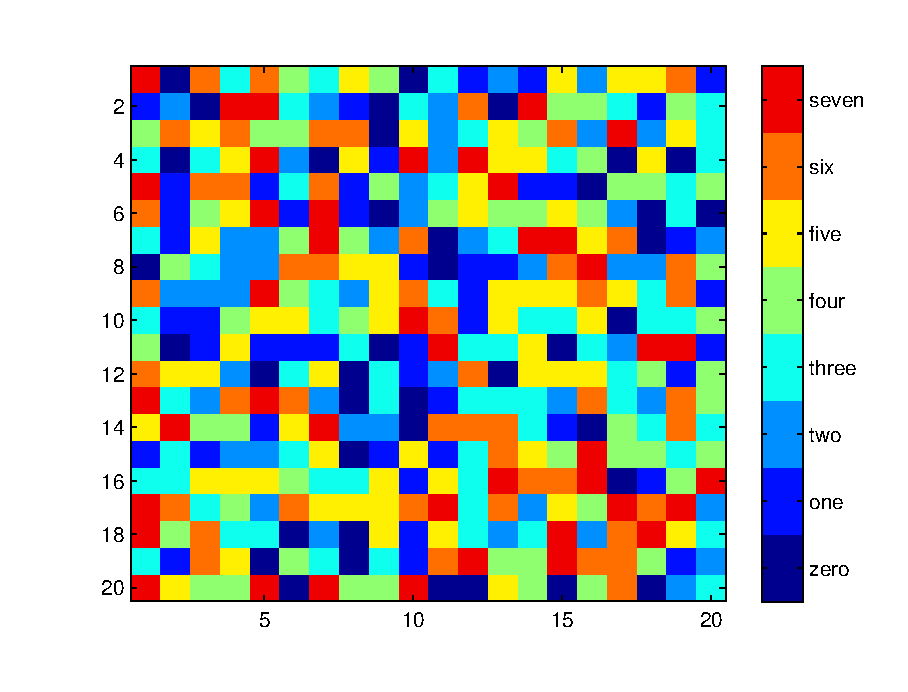
\includegraphics[scale = .9]{colorbar}
				\caption{Colorbar}
				\label{kap3:colorbar}
  		\end{center}
\end{figure}

% nebeneinander
\subsection{nebeneinder}
So lassen sich Bilder nebeneinander darstellen.
	\begin{figure}[!htbp]
		% TU Logo
  	\begin{minipage}{0.4\linewidth}
			\begin{center}
				
\includegraphics[scale=1]{tu-logo.eps}
  		\end{center}
  	\end{minipage}
		\hfill
		% EMSP Logo
  	\begin{minipage}{0.45\linewidth}
  		\begin{center}
				
\includegraphics[scale=0.3]{Logo_final.eps}
  		\end{center}
  	\end{minipage}
  	\caption{zwei Grafiken}
  	\label{kap3:neben}
	\end{figure}

\section{Diverses}
\subsection{Literaturverweise}

Einbinden von Verweisen: \cite{brig96}
Sieht im Text dann einfach wie \cite{Kamm02} aus.

\subsection{Verweise innerhalb des Dokuments}
Beispiele f�r Formeln gibt es in \ref{sec:formeln}

\subsection{Tabellen}

Beispiel f�r tabular-Umgebung

\begin{table}[!ht]
\caption[In Matlab]{Matlab-Befehle}
\label{tab:ML1}
\begin{tabular}{|| p{7cm} | p{6cm} ||} \hline\hline
I=eye(N);      																									& Einheitsmatrix \\ \hline
e=zeros(N,1); e(j)=1; 																					& Einheitsvektor\\ \hline
D=diag([d11,d22,...,dNN]); 																			& Diagonalmatrix \\ \hline
J=rot90(eye(N)); 																								& Koidentit�tsmatrix \\ \hline
E=ones(M,N); 																										& Einsmatrix \\ \hline
eins=ones(N,1); 																								& Einsvektor \\ \hline
t1=[t11,t12,...,t1N]; t2=[t11,t21,...,tN1]; 										& \\
T=toeplitz(t1,t2);  																						& Toeplitzmatrix \\ \hline
t=[t11,t12,...,t1N]; T=toeplitz(t); 														& symmetrische Toeplitzmatrix \\ \hline
x=[x1,x2,...,xN]; v=rot90(vander(x))'; 													& Vandermonde-Matrix \\ \hline
L=tril(A); 																											& untere Dreiecksmatrix der Matrix A \\ \hline
U=triu(A); 																											& obere Dreiecksmatrix der Matrix A \\ \hline\hline
\end{tabular}
\end{table}

\vspace*{2cm}

Das ganze nun mit longtable und hhline, aber ohne Beschriftung

\begin{longtable}{|| p{7cm} | p{6cm} ||} \hhline{||=|=||}
I=eye(N);       																								& {Einheitsmatrix} \\\hline
e=zeros(N,1); e(j)=1; 																					& Einheitsvektor\\ \hline
D=diag([d11,d22,...,dNN]); 																			& Diagonalmatrix \\ \hline
J=rot90(eye(N)); 																								& Koidentit�tsmatrix \\ \hline
E=ones(M,N); 																										& Einsmatrix \\ \hline
eins=ones(N,1); 																								& Einsvektor \\ \hline
t1=[t11,t12,...,t1N]; t2=[t11,t21,...,tN1]; 										& \\
T=toeplitz(t1,t2);  																						& Toeplitzmatrix \\ \hline
t=[t11,t12,...,t1N]; T=toeplitz(t); 														& symmetrische Toeplitzmatrix \\ \hline
x=[x1,x2,...,xN]; v=rot90(vander(x))'; 													& Vandermonde-Matrix \\ \hline
L=tril(A); 																											& untere Dreiecksmatrix der Matrix A \\ \hline
U=triu(A); 																											& obere Dreiecksmatrix der Matrix A \\ \hline\hline
\end{longtable}

	% Anhang
	\begin{appendix}
		% Anhang A - Quellcode

\chapter[Erstellter Programmcode]{Erstellter Programmcode}
%
F�r das Einf�gen erstellten Programmcodes bietet sich das Paket \textsl{listings} an. Der Funktionsumfang des Paketes ist sehr gro�, weshalb hier nur ein Beispiel gezeigt werden soll, dass mit den folgenden Einstellungen erzeugt wurde:
{\lstset{language=[LaTeX]{TeX}, basicstyle=\small, keywordstyle=\color{DarkBlue}}
\begin{lstlisting}
\lstset{language=Matlab, basicstyle=\small, xleftmargin=15pt,
        keywordstyle=\color{DarkBlue}, numbers=left, 
        numberstyle=\tiny, commentstyle=\color{DarkGreen}}.
\end{lstlisting}}
%
F�r weitere Informationen zu M�glichkeiten des Pakets sei auf dessen Dokumentation verwiesen.
\section{Matlab-Code}
% set style for matlab listings
\lstset{language=Matlab, basicstyle=\small, xleftmargin=15pt,
				keywordstyle=\color{DarkBlue}, numbers=left, 
				numberstyle=\tiny, commentstyle=\color{DarkGreen}}
%
Der folgende Code dient zur Erzeugung des Bildes \ref{kap3:colorbar}. Die Einr�ckungen im Quelltext sollen lediglich die M�glichkeiten des listings-Paket zeigen.

\begin{lstlisting}
%----------------------------------------------
% Make an image that uses only 8 levels/colors.
%----------------------------------------------
imagesc(floor(8*rand(20)))

%-----------------------------------------------------------
% Make an 8-row color map from the original 64-row colormap.
%-----------------------------------------------------------
	m64 = colormap; % Beispiel Einr�ckung
m8=m64(1:8:end,:);
	colormap(m8);   % Beispiel Einr�ckung

%---------------------
% Label new color map.
%---------------------
h = colorbar % Make colorbar and save handle.
set(h, 'ytick', (1:2:16)*7/16) % Assign positions of ticks
labels = strvcat('zero','one','two','three','four', ...
'five','six','seven'); %
%Make  levels for ticks.
set(h, 'yticklabel', labels) % Assign tick labels.
\end{lstlisting}


		% Anhang B - Scahltpl�ne

\chapter[Schaltpl�ne]{Schaltpl�ne}


		% Anhang A - Quellcode

\chapter[TeX-Editoren und Distributionen]{TeX-Editoren und Distributionen}

\section{TeXnicCenter}
Als frei verf�gbarer Editor f�r LaTeX-Projekte unter Windows ist TeXnicCenter in Verbindung mit der Distribution MiKTeX zu empfehlen. Hierbei sollte zuerst MiKTeX und anschlie�end TeXnicCenter installiert werden. Um die vorhandene Vorlage fehlerfrei kompilieren zu k�nnen, muss im TeXnicCenter ein bereits vordefiniertes Ausgabeprofil genutzt werden. Ausgabeprofile dienen dazu festzulegen, "`welches TeX"' (TeX, LaTeX, pdfTeX) benutzt wird und legen somit fest, in welchem Format verwendete Grafiken vorliegen m�ssen sowie das Format der Ausgabedatei. F�r weiterf�hrende Informationen sollten die entsprechenden Tutorials bem�ht werden.

\subsection{Ausgabeprofil f�r diese Vorlage}
F�r diese Vorlage kann das vordefinierte Ausgabeprofil LaTeX-->PS-->PDF genutzt werden. Auf diese Art und Weise ist es m�glich, eps-Grafiken einzubinden. Das Ergebnis des Kompilierens ist vorerst eine *.dvi-Datei. Diese wird danach automatisch zuerst in eine *.ps-Datei umgewandelt (mittels dvips.exe), welche anschlie�end in eine *.pdf-Datei konvertiert wird (ps2pdf.exe).

\subsection{Ausgabeprofile selbst Anlegen}
Manchmal kann es sinnvoll sein, eigene Ausgabeprofile zu definieren. Im folgenden wird ein Beispiel vorgestellt, mit dem ein Profil erzeugt wird, das im Projekt vor der Dokumentenklasse den Schalter "`$\backslash$ pdfoutput=0"' erwartet. Hierbei wird pdfTeX verwendet, aber eine *.dvi-Datei erzeugt, die anschlie�end nach pdf konvertiert werden soll.

Im TeXnicCenter ist unter dem Men�punkt \textit{Ausgabe} der Punkt \textit{Ausgabeprofile definieren} (auch ALT+F7) anzuw�hlen. Dort wird dann das vordefinierte Profil LATEX-->PDF kopiert und mit einem neuen, sinnvollen Namen versehen, z.\,B. Diplomarbeit. Die Registerkarten \textit{(La)TeX} und \textit{Viewer} k�nnen unver�ndert �bernommen werden. Unter \textit{Nachbearbeitung} werden nun zwei sogenannte Postprozessoren angelegt:

\begin{enumerate}

\item{DVIPS: Anwendung ist dvips.exe mit dem entsprechenden lokalen Pfad. Als Argument wird \textit{-R0 -P pdf ''\%Bm.dvi''} eingetragen.}

\item{PS2PDF: Anwendung ist gswin32c.exe (ghostview) ebenfalls mit dem entsprechenden lokalen Pfad. Als Argument wird \textit{-sPAPERSIZE=a4 -dSAFER -dBATCH -dNOPAUSE -sDEVICE=pdfwrite -sOutputFile=''\%bm.pdf'' -c save pop -f ''\%bm.ps''} angegeben.}

\end{enumerate}

Nun muss das soeben angelegte Profil noch aktiviert werden (Menu \textit{Auswahl/Aktives Ausgabeprofil w�hlen}). 

Der Vorlage liegt ein entsprechendes Beispielprofil (Datei TexnicCenterProfil.tco) bei, das importiert werden kann. Die lokalen Pfade zu den Anwendungen und Viewern m�ssen allerdings �berpr�ft bzw. per Hand erg�nzt werden.

\section{Weitere Editoren/Distributionen}
Es existiert eine Vielzahl weiterer Editoren zum Erstellen von TeX-Dokumenten. Beispiele hierf�r sind WinEdt, Winshell, LaTeX Editor oder auch LyX (wysiwyg). Eine �hnlich gro�e Auswahl herrscht bei TeX-Distributionen (z.\,B. teTeX, AucTeX, emTeX...). Eine gute �bersicht hierzu ist unter \url{http://www.math.vanderbilt.edu/~schectex/wincd/list_tex.htm} zu finden.
	\end{appendix}

	% das Abbildungsverzeichnis
	\listoffigures
	\addcontentsline{toc}{chapter}{Abbildungsverzeichnis}

	% das Tabellenverzeichnis
	\listoftables
	\addcontentsline{toc}{chapter}{Tabellenverzeichnis}

	% Literaturverzeichnis
	\raggedright													% Literatur im Flattersatz (v.a. wegen URLs)
	\bibliography{./Literatur/Literatur}
	\bibliographystyle{alphadin}

\end{document}
%%%%%%%%%%%%%%% END %%%%%%%%%%%%%%%









